\documentclass[12pt, a4paper]{article}

% Paquetes base
\usepackage[spanish, es-nodecimaldot]{babel}
\usepackage[utf8]{inputenc}
\usepackage[T1]{fontenc}
\usepackage{mathpazo}
\usepackage[margin=2.5cm]{geometry}
\usepackage{setspace}
\onehalfspacing
\usepackage{parskip}
\usepackage{microtype}
\usepackage{graphicx}
\usepackage{hyperref}
\hypersetup{colorlinks=true, linkcolor=black, urlcolor=blue, citecolor=black}
\usepackage{hyperref}
\usepackage{xcolor}
\usepackage{enumitem}
\usepackage{ragged2e}
\usepackage{float}
\usepackage{csquotes}
\usepackage{tabularx}
\usepackage{booktabs}
\usepackage{multirow}
\usepackage{amsmath}
\usepackage{amssymb}
\usepackage{caption}
\captionsetup{font=small} % Esto hace que todo el texto sea más pequeño


\usepackage{pgfplots}
\pgfplotsset{compat=1.18}

\usepackage{hyperref}
\hypersetup{
    colorlinks=false, % Desactiva el color del texto para activar los recuadros
    linkbordercolor=red, % Color del recuadro para \ref{} y el índice
    citebordercolor=green, % Color del recuadro para citas bibliográficas
    urlbordercolor=blue, % Color del recuadro para links web
    pdfborder={0 0 1} % El último número es el grosor de la línea del recuadro
}

% Configuración de espaciado y fuentes
\setstretch{1.1} % Espaciado interlineal ligeramente aumentado
\setlength{\parindent}{0pt} % Sin sangría en párrafos
\setlength{\parskip}{0.8em} % Espacio entre párrafos

%CITAS FORMATO APA 7

% Bibliografía APA 7
\usepackage[style=apa, backend=biber]{biblatex}
% Asegúrate de tener un archivo llamado referencias.bib
\addbibresource{referencias.bib} 

% Añade esto después de \addbibresource{referencias.bib}
\DefineBibliographyExtras{spanish}{%
  \restorecommand\mkbibnamefamily
  \restorecommand\mkbibnamegiven
  \let\finalandcomma=\empty
  \let\finalandsemicolon=\empty
}

\DefineBibliographyStrings{spanish}{
  and = {y},
  andothers = {y otros},
  references = {Referencias}
}

% Encabezado/pie
\usepackage{fancyhdr}
\pagestyle{fancy}
\fancyhf{}

% Altura del encabezado para que quepa el logo (1.8 cm ~ 51pt)
\setlength{\headheight}{52pt}
% (Opcional) si ves el contenido muy abajo, puedes recuperar un poco de margen:
% \addtolength{\topmargin}{-8pt}

% Encabezado
\lhead{
\includegraphics[height=1.8cm]{escudo.png}}
\chead{Universidad del Bío-Bío}
\rhead{\nouppercase{\leftmark}}

% Pie de página
\lfoot{Sistemas Digitales}
\cfoot{\thepage}
\rfoot{Grupo 8}

% Líneas superior e inferior
\renewcommand{\headrulewidth}{0.4pt}
\renewcommand{\footrulewidth}{0.4pt}

% Espaciado de títulos (aleja los títulos del encabezado)
\usepackage{titlesec}
\titlespacing*{\section}{0pt}{2cm}{-0.1cm}

% (Opcional) Sin numeración en títulos (y siguen en el índice)
\setcounter{secnumdepth}{0}

% (Opcional) Cambiar el nombre del índice a "Índice"
\addto\captionsspanish{\renewcommand{\contentsname}{Índice}}
\setlength{\footskip}{0.9cm}  % valor más chico → sube el pie



\begin{document}
	
	\begin{titlepage}
		\thispagestyle{empty}
		
		% ===== Bloque superior: escudo + institución =====
		\begin{center}
			\vspace*{-2cm} % margen superior discreto
			
\includegraphics[height=3.5cm]{escudo.png}\\[-0.2cm]
			
			{\large Universidad del Bío-Bío}\\[-2pt]
			{\large Facultad de Ciencias Empresariales}\\[-2pt]
			{\large Ingeniería Civil en Informática}
		\end{center}
		
		\vspace{1cm}
		\vfill
		
		% ===== Bloque central: TÍTULO =====
		\begin{center}
			\rule{\textwidth}{0.5pt}\\[0.5cm]
			{\Huge \textbf{Informe de laboratorio N\textsuperscript{o}1}}\\[0.25cm]
			{\Large Convertidor Analógico - Digital}\\[0.1cm]
			\rule{0.65\textwidth}{0.5pt}
		\end{center}
		
		\vspace{2cm}
		
		% ===== Bloque inferior compacto: Asignatura, Profesor, Integrantes =====
    \begin{flushleft}
    \normalsize
    \begin{tabular}{@{}ll@{}}
                           & \\
    \textbf{Integrantes}   & : Oscar Illanes Garrido \\
                           & \hspace{0.12 cm} Gabriela Maureira Ocaña \\
                           & \hspace{0.12 cm}  Bastian Palma Navarrete \\
                           & \\
    \textbf{Docente}       & : Julio C. Alarcón Monteros \\
                           & \\
    \textbf{Asignatura}    & : Sistemas Digitales \\
                           & \\
    \textbf{Carrera}    & : Ingeniería Civil en Informática \\
    \end{tabular}
    \end{flushleft}
		
		\vfill
		\begin{center}
			\normalsize\textbf{Chillán, 10 de abril de 2026.}
		\end{center}
	\end{titlepage}
	
	\tableofcontents 

	\newpage
	
	\section{Introducción}

    Es común preguntarse cómo las señales físicas del mundo real -como la voz humana al hablar por un micrófono o las variaciones de temperatura- logran transformarse en los datos que procesan nuestras computadoras. Para responder a esta interrogante, en este primer laboratorio se abordó el diseño de un Convertidor Analógico-Digital (ADC), un sistema que sirve como el ejemplo perfecto de cómo estas magnitudes continuas se traducen al lenguaje binario que sustenta la tecnología actual.

    Para facilitar su lectura, el documento se divide en distintas secciones. Se comienza con la definición de los objetivos planteados, seguido del desarrollo teórico que sirvió como base para la actividad. El núcleo del trabajo se encuentra en la sección de "Diseño del sistema digital", donde se exponen conceptos clave, desarrollo matemático argumentativo y representaciones gráficas para una mejor comprensión.

    Es importante tener en cuenta ciertas consideraciones metodológicas. A lo largo del texto se emplea lenguaje técnico para definir los conceptos. Además, debido a los requerimientos del laboratorio, la simulación se llevó a cabo en Multisim, por lo que los datos analizados asumen condiciones ideales de operación.

    Finalmente, el informe concluye con un análisis experimental en el que se exploran los resultados obtenidos y se comparan con los valores esperados teóricamente.

	\section{Objetivos}

    \subsection{Objetivo General:}
    \begin{itemize}
        \item Comprender y validar el proceso de digitalización de una señal analogica mediante el diseño y simulación de un circuito convertidor analogico-digital
    \end{itemize}

    \subsection{Objetivos específicos:}
    \begin{itemize}
        \item Determinar las características de digitalización de una señal analógica senoidal de 50hz operando en un rango de -12 a +12 volt.
        \item Diseñar y simular un circuito ADC para la señal analogica utilizando el software Mltisim, visualizando la salida mediante un display de LEDs
        \item Comprobar empíricamente la relación teórica entre el voltaje de entrada y el código binario de salida contrastando éstos con los datos obtenidos. 
    \end{itemize}

    \newpage

    \section{Desarrollo teórico}

    El proceso de convertir una cantidad analógica a digital en el mundo físico comienza generalmente con el uso de un transductor, dispositivo encargado de convertir una magnitud física en una señal eléctrica analógica proporcional. Una vez obtenida esta señal, el estudio se centra en el \textbf{convertidor analógico-digital (ADC)}, el cual actúa como el componente esencial para transformar dichas señales (voltajes, intensidades entre otros) continuas en representaciones binarias discretas.
    
    Es fundamental definir que, según \cite{floyd2006fundamentos} considera una magnitud analógica como aquella que toma valores continuos, mientras que una magnitud digital toma un conjunto de valores discretos. En la práctica, la mayoría de cosas que se pueden medir cuantitativamente aparecen naturalmente de forma analógica. Por ejemplo, en la Figura \ref{fig:GrafAnalogica} se representan voltajes durante un rango continuo de tiempo.

        \begin{figure}[H]
        \centering
        \begin{tikzpicture}[scale=0.6]
            \begin{axis}[
                width=15cm, height=8cm,
                % Nuevos rangos solicitados
                xmin=0, xmax=15.5,
                ymin=0, ymax=7,
                % Configuración de ejes
                axis lines=left,
                xlabel={t (s)},
                ylabel={voltaje (v)},
                ylabel style={at={(0,1)}, rotate=-90, anchor=south},
                xlabel style={at={(1,0)}, anchor=west},
                % Cuadrícula (Grid)
                grid=both,
                major grid style={line width=.2pt,draw=gray!50},
                % Marcas del eje X de 1 a 15
                xtick={1,2,3,4,5,6,7,8,9,10,11,12,13,14,15},
                % Marcas del eje Y de 1 a 10
                ytick={1,2,3,4,5,6,7},
                tick style={draw=none}
            ]

                % Curva escalada para mantener la forma original en el nuevo rango
                % X original (0-24) -> X nuevo (0-15)
                % Y original (19-26.5) -> Y nuevo (1-9 approx)
                \addplot[
                    smooth,
                    thick,
                    color=black,
                ] plot coordinates {
                    (0, 1.8) (1.8, 1.5) (3.1, 1.1) (4.3, 1.6) (5.6, 3.5) 
                    (6.8, 5.3) (8.4, 6.1) (10, 5.5) (11.8, 3.3) (13.1, 1.9) (15, 1.2)
                };

            \end{axis}
        \end{tikzpicture}
        \caption{Representación gráfica de una señal analógica}
        \label{fig:GrafAnalogica}
    \end{figure}

    Un ADC no puede proporcionar una representación binaria para los infinitos puntos que componen la gráfica [Figura \ref{fig:GrafAnalogica}] ya que es inviable computacionalmente. Por esto es que digitaliza mediante un proceso de muestreo, el cual consta de tomar un número suficiente de valores discretos en determinados periodos de tiempo (eje $x$) de una forma de onda como para poder definir adecuadamente esa forma de onda \parencite{floyd2006fundamentos}. Como consecuencia de lo anterior, se obtiene la Figura \ref{fig:GrafCuantificada}.

    \begin{figure}[H]
        \centering
        \begin{tikzpicture}[scale=0.6]
        \begin{axis}[
            width=15cm, height=8cm,
            % Forzamos que los límites sean exactos
            xmin=0, xmax=15.5,
            ymin=0, ymax=7,
            % IMPORTANTE: Desactiva el desplazamiento automático de los ejes
            enlarge x limits=false,
            axis lines=left,
            xlabel={t (s)},
            ylabel={voltaje (v)},
            ylabel style={at={(0,1)}, rotate=-90, anchor=south},
            xlabel style={at={(1,0)}, anchor=west},
            grid=both,
            major grid style={line width=.2pt,draw=gray!50},
            % Definimos ticks desde 0 para que la cuadrícula sea perfecta
            xtick={0,1,2,3,4,5,6,7,8,9,10,11,12,13,14,15},
            % Pero solo mostramos las etiquetas desde el 1
            xticklabels={,1,2,3,4,5,6,7,8,9,10,11,12,13,14,15},
            ytick={1,2,3,4,5,6,7},
            tick style={draw=none},
            ycomb,
        ]

            \addplot[
                fill=black,
                draw=black,
                mark=*,
                mark size=2pt,
                thick,
            ] coordinates {
                (1, 1.63) (2, 1.41) (3, 1.12) (4, 1.45) 
                (5, 2.76) (6, 4.19) (7, 5.42) (8, 6.01) (9, 5.86) 
                (10, 5.50) (11, 4.23) (12, 3.01) (13, 2.01) (14, 1.57) (15, 1.20)
            };

        \end{axis}
        \end{tikzpicture}
        \caption{Representación de los voltajes muestreados de la Figura \ref{fig:GrafAnalogica}}
        \label{fig:GrafCuantificada}
    \end{figure}

    \newpage

    Cuando hay que muestrear una señal analógica, es necesario satisfacer ciertos criterios para poder representar de manera precisa la señal original.
    \begin{itemize}
        \item \textbf{Teorema del muestreo (Nyquist-Shannon):} Establece que para poder representar una señal analógica discretizada sin pérdida de información, la frecuencia de muestreo ($f_{s}$), debe ser al menos dos veces superior a la componente de mayor frecuencia ($f_{max}$) de la señal analógica.  
    \end{itemize}

    \begin{equation}
        f_{s} \geq 2f_{max}
        \label{eq:nyquist}
    \end{equation}

    Una analogía simple que nos permite comprender este teorema es imaginarse una pelota en movimiento, la cual se quiere fotografiar. Si se toma una única fotografía, no es posible extraer información sobre el comportamiento de la pelota. Al incrementar el número de capturas en instantes  equiespaciados, permite determinar con mayor precisión la trayectoria seguida durante el rebote. Este concepto se traslada directamente al procesamiento de señales mediante el Teorema de Nyquist-Shannon antes mencionado.

    Una vez realizado en proceso de muestreo bajo los criterios de Nyquist, se procede a la cuantificación, \cite{floyd2006fundamentos} establece la cuantificación como \enquote{el proceso de convertir la salida del circuito de muestreo en una serie de códigos binarios que representan la amplitud de la entrada analógica en cada uno de los instantes de muestreo}. En otras palabras es designarle un valor binario a los intervalos de voltajes muestreados (eje $y$), en la Figura \ref{img:13.1} se puede apreciar como se ilustra la cuantificación de una onda analógica en cuatro niveles (2 bits). Además de una onda representada con forma de \enquote{escalera}, esto es resultado de mantener el voltaje constante (retención) para que el ADC pueda asignar el código binario sin errores por variaciones de la señal.
    
    \begin{figure}[H]
        \centering
        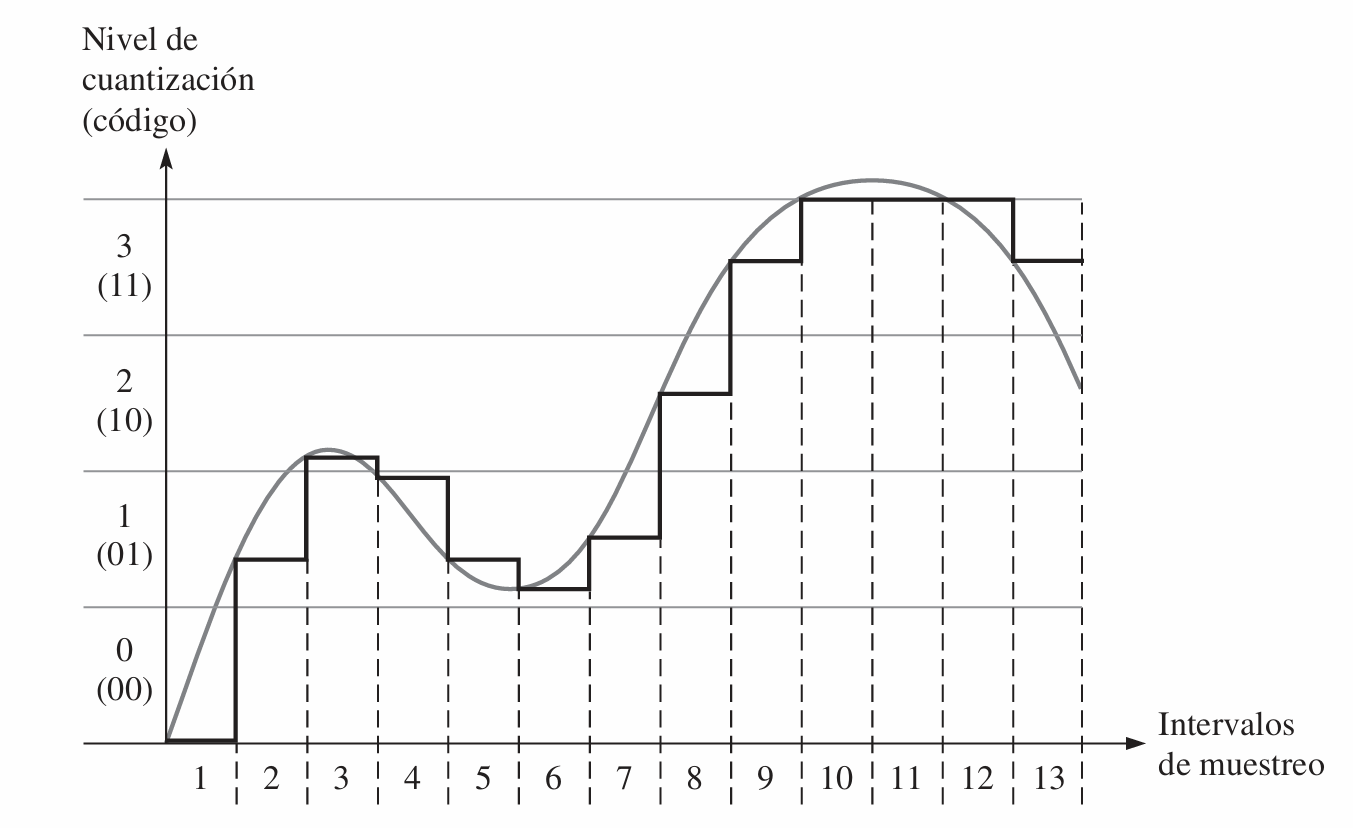
\includegraphics[width=0.8\textwidth]{Fig13.1.png}
        \caption{Forma de onda de salida con cuatro niveles de cuantificación \parencite[p. 842]{floyd2006fundamentos}.}
        \label{img:13.1}
    \end{figure}

    \newpage

    La precisión con la que el ADC representa una señal analógica está determinada por su resolución, concepto que define el cambio mínimo de voltaje necesario para provocar un cambio en el código binario de salida. Este parámetro se manifiesta físicamente como el voltaje de resolución o tamaño del escalón de cuantización, y se calcula dividiendo el rango total de voltaje de entrada ($V_{ref+} - V_{ref-}$) por el número total de niveles discretos que el convertidor puede generar ($2^n$, donde $n$ es el número de bits).

    En un sistema donde se emplean más bits, este voltaje de resolución disminuye, lo que permite que los escalones de la Figura \ref{img:13.1} sean más pequeños y, por lo tanto, la aproximación a la señal original sea mucho más exacta. Por el contrario, un voltaje de resolución muy elevado genera un error de cuantización más notorio, Este error se define formalmente como la diferencia entre el valor de voltaje analógico real presente en la entrada y el valor discreto asignado por el ADC, el error de cuantización máximo es de $\pm \frac{1}{2} LSB$ (o la mitad del voltaje de resolución).

    Como se observa en la Figura \ref{img:13}, el proceso de cuantificación culmina con la generación de una salida digital que representa la magnitud de la señal analógica original. En esta etapa, el convertidor traduce los niveles de voltaje escalonados en una serie de códigos binarios, los cuales se manifiestan como un tren de pulsos lógicos.

    \begin{figure}[H]
        \centering
        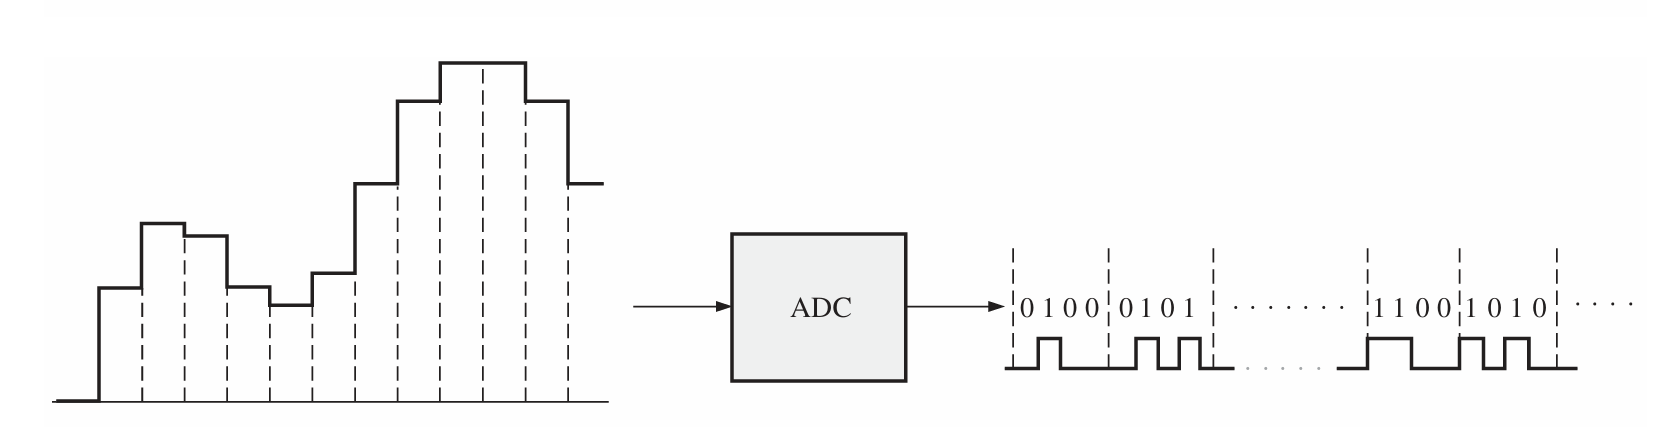
\includegraphics[width=1\textwidth]{Fig13.png}
        \caption{Representación de codificación de un convertidor analógico-digital \parencite[p. 842]{floyd2006fundamentos}}
        \label{img:13}
    \end{figure}


	\newpage

    \section{Diseño del sistema digital}

    Para el desarrollo del sistema de conversión analógico-digital, se definió un esquema basado en bloques funcionales, el cual permite representar de manera clara el funcionamiento general del sistema sin necesidad de mostrar el circuito implementado en el software de simulación Multisim. Este enfoque facilita la comprensión del proceso de conversión desde la señal analógica hasta su representación digital.

    El sistema está compuesto por los siguientes bloques principales:
    \begin{itemize}
        \item Generador de señal senoidal (entrada analógica)
        \item Convertidor Analógico-Digital (ADC de 8 bits)
        \item Generador de señal de muestreo
        \item Sistema de visualización de salida digital (LEDs)
    \end{itemize}

    La señal de entrada corresponde a una señal eléctrica analógica de tipo senoidal, con un rango de -12V a 12V y una frecuencia de 50 Hz. Esta señal es aplicada a la entrada del ADC, el cual convierte el valor instantáneo del voltaje en un código binario de 8 bits.

    Por otra parte, el generador de señal de muestreo entrega una señal cuadrada de 1000 Hz, la cual determina los instantes en que se realiza cada conversión. Finalmente, la salida digital es representada mediante un conjunto de LEDs, que permiten visualizar el código binario generado.

    \subsection{Esquema general del sistema}

    El funcionamiento del sistema se puede representar mediante el siguiente diagrama de bloques:

    \begin{figure}[H]
        \centering
        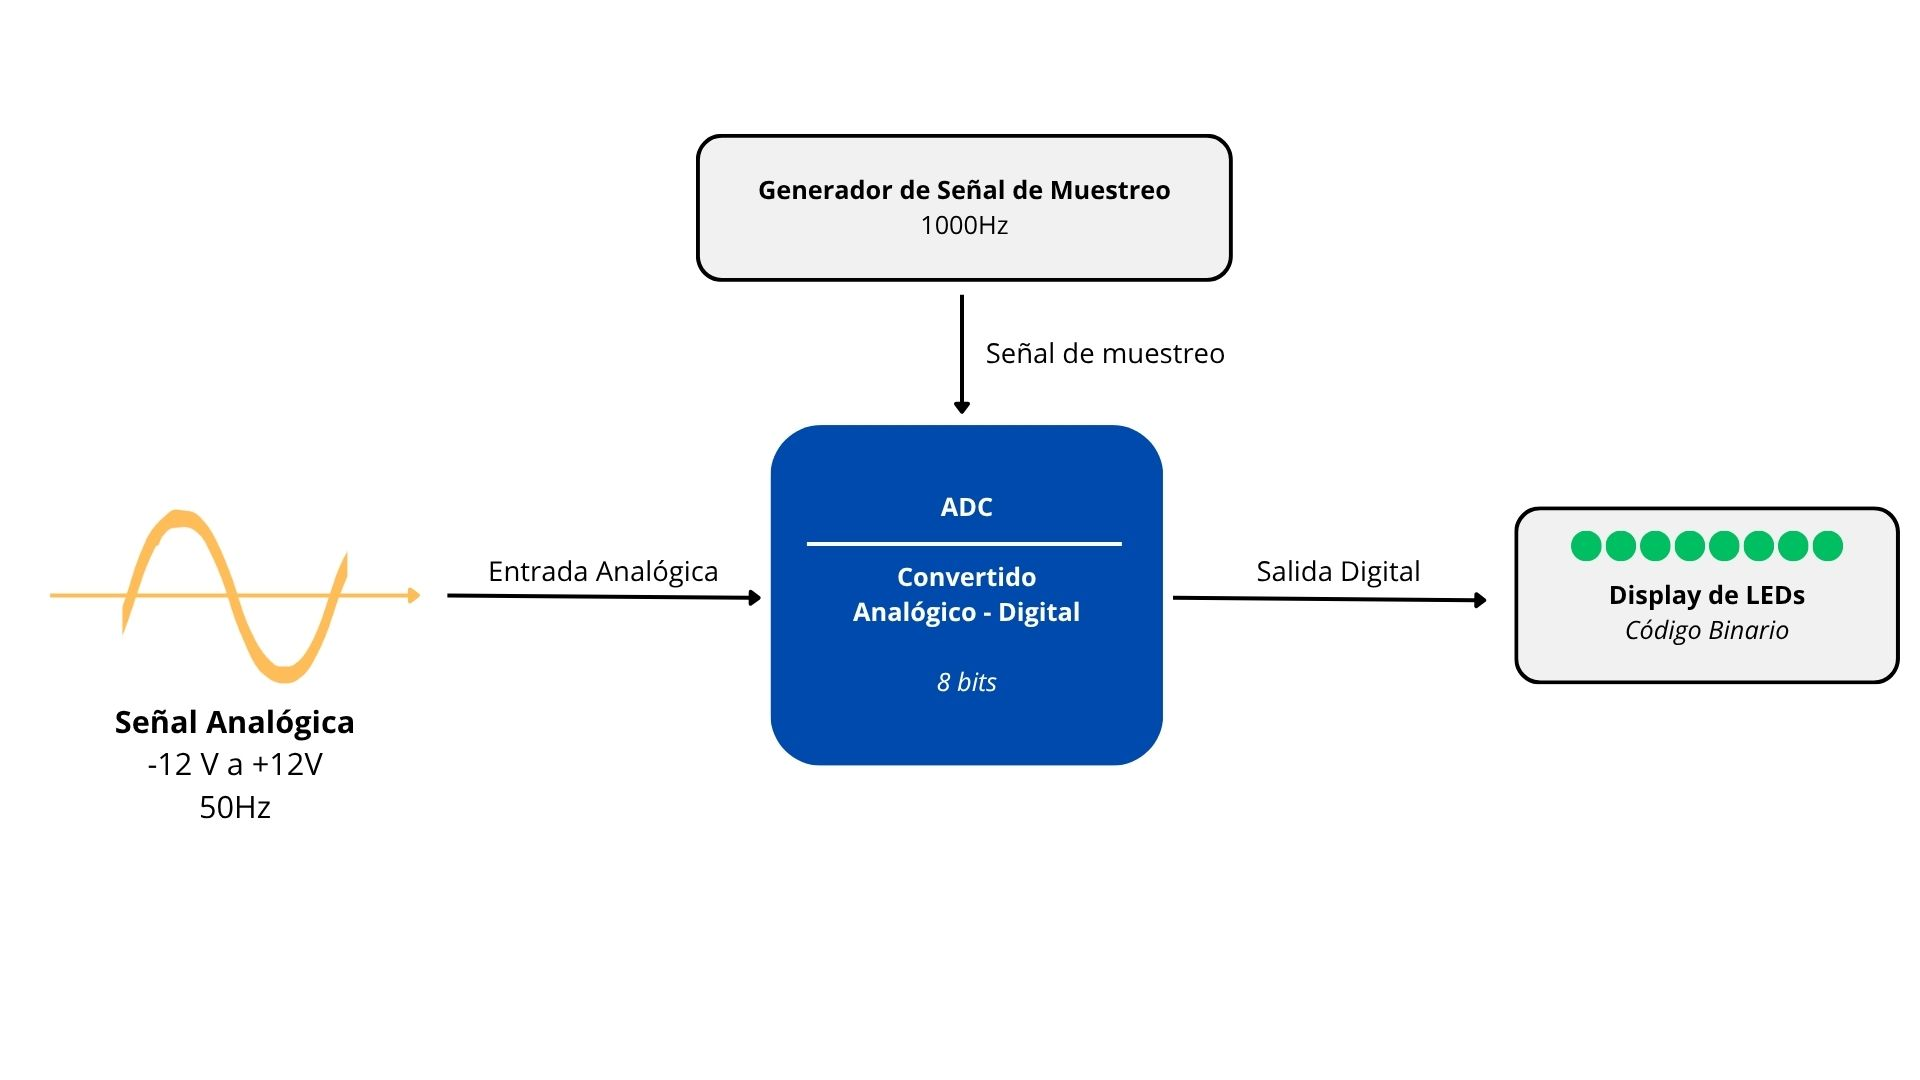
\includegraphics[width=0.7\linewidth]{ADC Convertido Analógico - Digital 8 bits (1).jpg.jpeg}
        \caption{Esquema general correspondiente a la simulación.}
        \label{img:EsquemaGen}
    \end{figure}

    \newpage

    En la Figura \ref{img:EsquemaGen} se observa que la señal analógica es aplicada al ADC, mientras que la señal de muestreo define los instantes en los cuales se realiza la conversión. Como resultado, se obtiene una salida digital que corresponde a un valor binario proporcional al voltaje de entrada en cada instante de muestreo.

    \subsection{Resolución del ADC}

    Para analizar el comportamiento del sistema, se calcula la resolución del convertidor, la cual corresponde al cambio mínimo de voltaje que puede ser representado:

    \begin{equation}
        V_{res} = \frac{V_{max} - V_{min}}{2^n}
        \label{eq:Vres}
    \end{equation}

    Donde:

    \begin{itemize}
        \item $V_{max} = 12V$
        \item $V_{min} = -12V$
        \item $n = 8 \text{ bits}$
    \end{itemize}

    Reemplazando:

    $$ V_{res} = \frac{12-(-12)}{256} = 0.09375V $$

    De acuerdo con la ecuación \ref{eq:Vres}, cada incremento en el valor digital representa aproximadamente 0.09375 V, lo que define la precisión del sistema.

    \subsection{Frecuencia de muestreo}

    De acuerdo con lo solicitado, el sistema debe realizar 20 muestras por cada ciclo de la señal senoidal. Para ello, se utiliza la siguiente relación:
    \begin{equation}
        f_s = f \times N 
        \label{eq:freq_muestreo}
    \end{equation}

    Donde:
    \begin{itemize}
        \item $f = 50 \text{ Hz}$
        \item $N = 20 \text{ muestras}$
    \end{itemize}

    $$ f_s = 50 \times 20 = 1000 \text{ Hz} $$

    Según la ecuación \ref{eq:freq_muestreo}, la frecuencia de muestreo del sistema es de 1000 Hz, lo que asegura una adecuada representación de la señal de entrada (por teorema del muestreo).

    \subsection{Relación entre el voltaje de entrada y la salida digital}

    La relación entre el voltaje de entrada y el valor digital generado por el ADC se puede expresar mediante la siguiente ecuación:

    \begin{equation}
        D_{10} = \frac{V_{in} - V_{min}}{V_{res}}
        \label{eq:D10}
    \end{equation}

    Donde:
    \begin{itemize}
        \item $D_{10}$: Valor decimal
        \item $V_{in}$: Voltaje de entrada
        \item $V_{min}$: Voltaje de referencia mínimo (-12V)
        \item $V_{res}$: Voltaje de resolución (0.09375V)
    \end{itemize}

    Reemplazando:

    $$ D_{10} = \frac{V_{in} - (-12)}{0.09375} $$

    Esta ecuación (\ref{eq:D10}) permite determinar el código decimal asociado a los valores de entrada dentro del rango de operación del ADC.

    \subsection{Resultados esperados}

   A partir del análisis teórico, se espera que el ADC genere un código binario proporcional al voltaje de entrada. En particular:

    \begin{itemize}
        \item Para $V_{in} \approx -12V \rightarrow 00000000$
        \item Para $V_{in} \approx 0V \rightarrow 10000000$
        \item Para valores intermedios $\rightarrow$ Aumento progresivo
        \item Para $V_{in} \approx 12V \rightarrow 11111111$
    \end{itemize}

    Además, se espera que la señal digital resultante presente una forma escalonada, producto del proceso de cuantización propio del ADC.

    \newpage

    Como ejemplo, para un voltaje de entrada ($V_{in}$) = \textbf{2.5 V} y utilizando la ecuación \ref{eq:D10} :

    $$ D_{10} = \frac{2.5 + 12}{0.09375} = \frac{14.5}{0.09375} \approx 154.67 $$

    El valor se trunca a 154, ya que el ADC no realiza redondeo sino cuantización por niveles discretos.
    El valor decimal 154 corresponde al código binario: \textbf{10011010}

    Este resultado es coherente con el comportamiento esperado del ADC y permite su comparación con los valores obtenidos en la simulación, verificando así el correcto funcionamiento del sistema diseñado.



    \subsection{Análisis del diseño}

    El sistema diseñado permite convertir una señal analógica en una señal digital de forma adecuada, cumpliendo con el funcionamiento esperado de un ADC.

    La resolución del ADC define qué tan preciso es el sistema, ya que indica el cambio mínimo de voltaje que se puede representar. Debido a esto, existe un pequeño error llamado cuantización, ya que no todos los valores analógicos pueden representarse exactamente.

    Por otra parte, la frecuencia de muestreo utilizada (1000 Hz) permite tomar suficientes muestras de la señal en cada ciclo, lo que asegura que su forma senoidal se represente de buena manera.

    Además, se observa que la salida digital aumenta a medida que aumenta el voltaje de entrada, lo que demuestra que el sistema funciona de forma coherente.

    En conjunto, este análisis permite tener una base para comparar con los resultados de la simulación y comprobar que el sistema funciona correctamente.

    \newpage

    \section{Simulación del circuito}

    A continuación, se presenta la simulación del circuito diseñado anteriormente, la cual fue realizada utilizando el software Multisim. El objetivo de esta etapa es verificar el correcto funcionamiento del sistema y comparar los resultados obtenidos con el análisis teórico.

    El circuito implementado se muestra en la figura 6. En este, se utilizó una fuente de señal senoidal configurada con un rango de -12 V a 12 V y una frecuencia de 50 Hz, representando la señal de entrada. Además, se incorporó un generador de señal cuadrada de 1000 Hz, el cual actúa como señal de muestreo.

    Antes de adentrarse en la simulación del circuito es fundamental definir los elementos más importantes que conforman al convertidor analógico-digital (ADC):

    \begin{itemize}
        \item \textbf{$ V_{in} $ (voltaje de entrada):} Es la señal analógica continua que proviene del transductor, en el circuito esta terminal está conectada a una fuente de $AC_VOLTAGE$ configurada a 12Vpk y 50 Hz.
        \item \textbf{ $V_{ref+}$ (voltaje de referencia máxima): } Esta entrada define el rango máximo del ADC. En la simulación, $V_{ref+}$ se conecta a una fuente VCC de $12\text{ V}$
        \item \textbf{ $V_{ref-}$ (voltaje de referencia mínimo):} Esta entrada definen el rango mínimo del ADC. En la simulación, $V_{ref-}$ se conecta a una fuente a una fuente VDD de $-12\text{ V}$ 
        \item \textbf{SOC (Start of Conversion):} Este puerto recibe la señal de un reloj digital (\texttt{DIGITAL\_CLOCK}) ajustado a una frecuencia ($f_s$) de $1000\text{ Hz}$. Esta conexión es fundamental para dictar el ritmo del muestreo, cumpliendo con el criterio de obtener 20 muestras por ciclo de la señal de entrada.
        \item \textbf{D0-D7P} La salida digital se obtiene a través de los terminales D0 a D7, los cuales se conectan a una barra de 8 LEDs para visualizar el código binario generado. 
    \end{itemize}


    \begin{figure}[H]
        \centering
        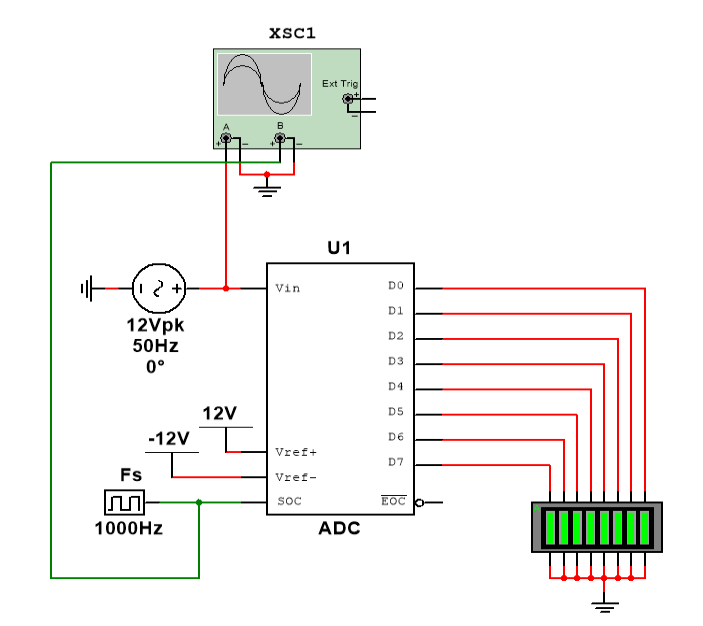
\includegraphics[width=0.6\textwidth]{SimulacionMultisim.png}
        \caption{Circuito en Multisim}
        \label{img:Multisim}
    \end{figure}

    \subsection{Verificación de la frecuencia de muestreo}

    Para comprobar que el sistema realiza 20 muestras por ciclo, se simuló un período completo de la señal de entrada y se observaron los pulsos del reloj en el osciloscopio.

    \begin{figure}[H]
        \centering
        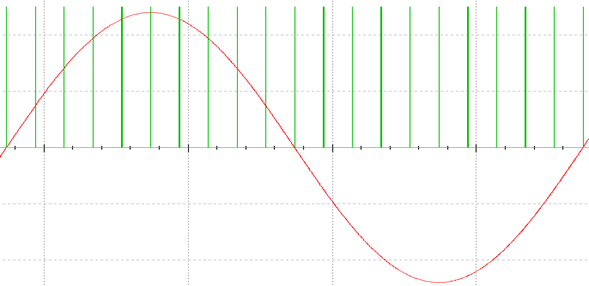
\includegraphics[width=0.6\textwidth]{Onda.png}
        \caption{Frecuencia de muestreo correspondiente a la onda senoidal}
        \label{img:OndaSenoidal}
    \end{figure}

    En la Figura \ref{img:OndaSenoidal}  se visualiza la señal analógica en color rojo, correspondiente al canal A, y la señal de muestreo en color verde, correspondiente al canal B. Al analizar el intervalo que corresponde a un período completo de la señal senoidal, es posible identificar la cantidad de pulsos generados por la señal de muestreo.

    Al realizar este análisis, se determinó que dentro de un ciclo completo se presentan 20 pulsos, lo cual coincide con lo establecido en el diseño del sistema. Esto confirma que la frecuencia de muestreo utilizada permite obtener la cantidad de muestras requeridas para representar adecuadamente la señal de entrada.

    Para respaldar esta observación, es necesario considerar la configuración del osciloscopio utilizada durante la simulación, en particular:

    \begin{itemize}
        \item Base de tiempo: 5 ms/Div
        \item Canal A (señal analógica): 5 V/Div
        \item Canal B (señal de muestreo): 2 V/Div
    \end{itemize}

    La base de tiempo de 5 ms/Div indica que cada división horizontal en la pantalla del osciloscopio representa 5 milisegundos. Esto permite visualizar un período completo de la señal senoidal, considerando que su período es de 20 ms (correspondiente a una frecuencia de 50 Hz).

    Por otra parte, la escala del canal A de 5 V/div significa que cada división vertical equivale a 5 volts, lo que permite observar correctamente la amplitud de la señal analógica en el rango de -12 V a 12 V.

    En el caso del canal B, una escala de 2 V/div permite visualizar de forma clara los pulsos de la señal de muestreo, facilitando su conteo dentro del período de la señal.

    Gracias a esta configuración, es posible identificar de manera precisa tanto la duración de un ciclo como la cantidad de pulsos presentes en este, lo que permite validar que el sistema cumple con las 20 muestras por ciclo definidas en el diseño.

    \subsection{Verificación del funcionamiento del ADC}

    Una vez comprobado que el sistema realiza correctamente las 20 muestras por ciclo, se procedió a verificar que el circuito es capaz de convertir adecuadamente la señal analógica en una señal digital.

    Para esto, se analizaron distintos puntos de la señal de entrada, deteniendo la simulación en momentos específicos para medir el voltaje de entrada y observar la salida digital entregada por el ADC. Posteriormente, estos valores fueron comparados con los resultados esperados utilizando la ecuación (4).

    Con el fin de evaluar correctamente el comportamiento del sistema, se seleccionaron cinco situaciones representativas de la señal:

    \subsection{\textit{Caso 1: Maximo}}

    Para este caso se configuro la simulación para detenerse a los 0.0251 segundos, esto debido a que la frecuencia de la señal es de $50 \text{ Hz}$, es decir  el periodo ($T$) es de $20 \text{ ms}$ y el pico máximo muestreado ocurre al primer cuarto del segundo ciclo. El resultado se puede apreciar en la Figura \ref{img:maximo}.

    \begin{figure}[H]
        \centering
        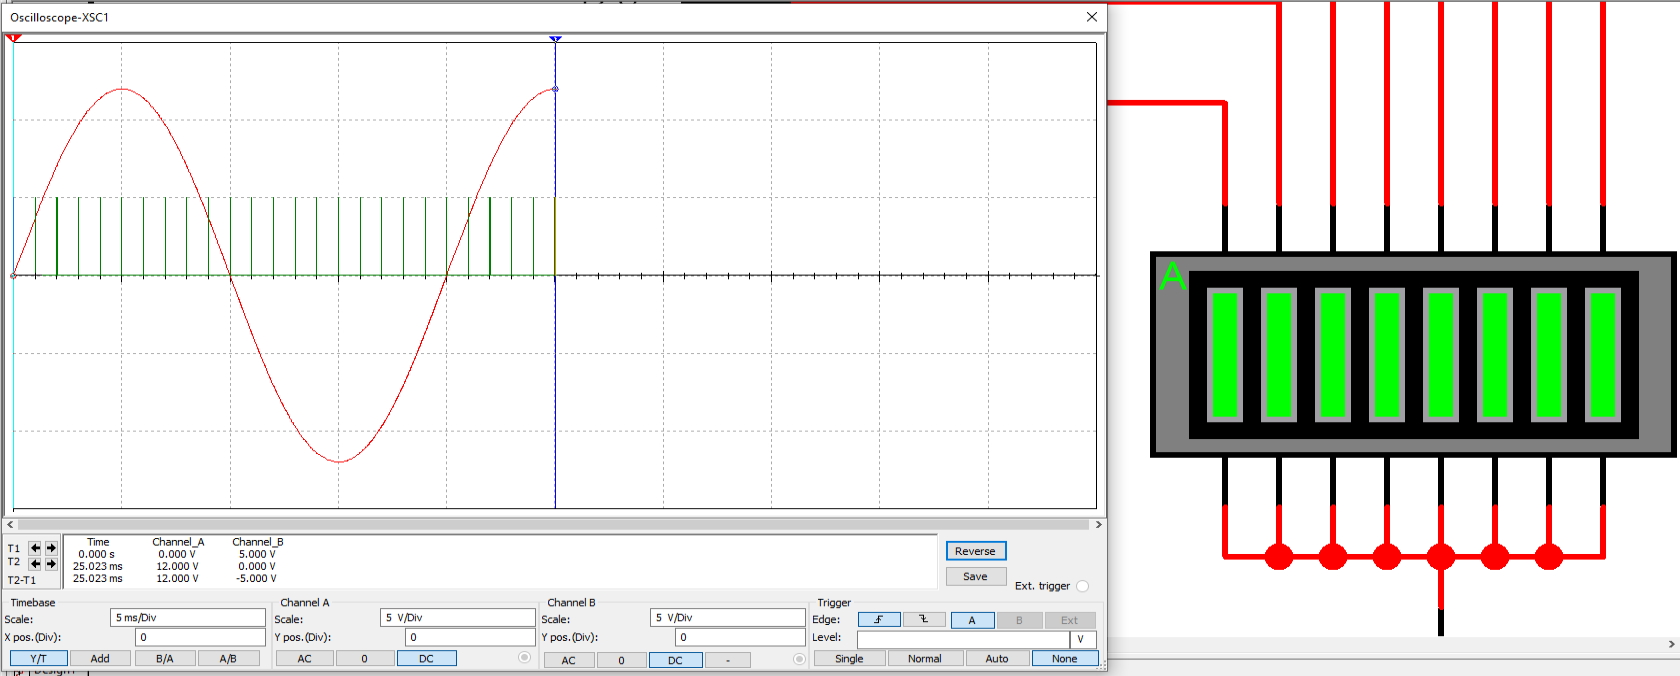
\includegraphics[width=1\textwidth]{Maximo.png}
        \caption{Onda senoidal del Multisim en su pico mas alto (12V)}
        \label{img:maximo}
    \end{figure}

    Podemos notar que el voltaje obtenido de la simulación esta dada por T2 en el channel\_A, el cual corresponde al valor de 12V concordando efectivamente con $V_{ref+}$. Según los LEDs el valor asignado para 12V es de \textbf{11111111} (8 bits encendidos), para verificar este código se utilizara la ecuación (\ref{eq:D10}) planteada anteriormente:

    De acuerdo con los datos del diseño:
    \begin{itemize}
        \item Voltaje de entrada ($V_{in}$): $12\text{ V}$ 
        \item Voltaje de referencia mínimo ($V_{min}$): $-12\text{ V}$
        \item Voltaje de resolución ($V_{res}$): $0.09375\text{ V}$
    \end{itemize}

    $$D_{10} = \frac{12 - (-12)}{0.09375} = \frac{24}{0.09375} = 256$$
    
    Notar que el valor decimal de 256 convertido a binario corresponde a \textbf{100000000} el cual es de 9 bits. Dado que el convertidor analógico-digital es de $n = 8$ bits, el rango de salida está limitado a un valor máximo de $2^n - 1$, es decir, un intervalo de $[0, 255]$. Por lo tanto, el valor decimal se satura en el límite superior (255).

    $$255_{10} = 11111111_2$$

    El codigo binario calculado coincide con la visualización de la simulación en Multisim, donde se observan los 8 LEDs de la barra encendidos. Esto valida que el ADC está en un funcionamiento correcto para el límite superior de voltaje ($V_{ref+}$)
    
    
    \subsection{\textit{Caso 2: minimo}}

    Para el voltaje \textbf{mínimo}, se volvió a configurar la simulación, esta vez para detenerse a los 0.0151 segundos, bajo la misma lógica se dedujo que el pico mas bajo ocurriría al tercer cuarto del primer ciclo. El resultado se puede apreciar en la Figura \ref{img:minimo}.
    
    \begin{figure}[H]
        \centering
        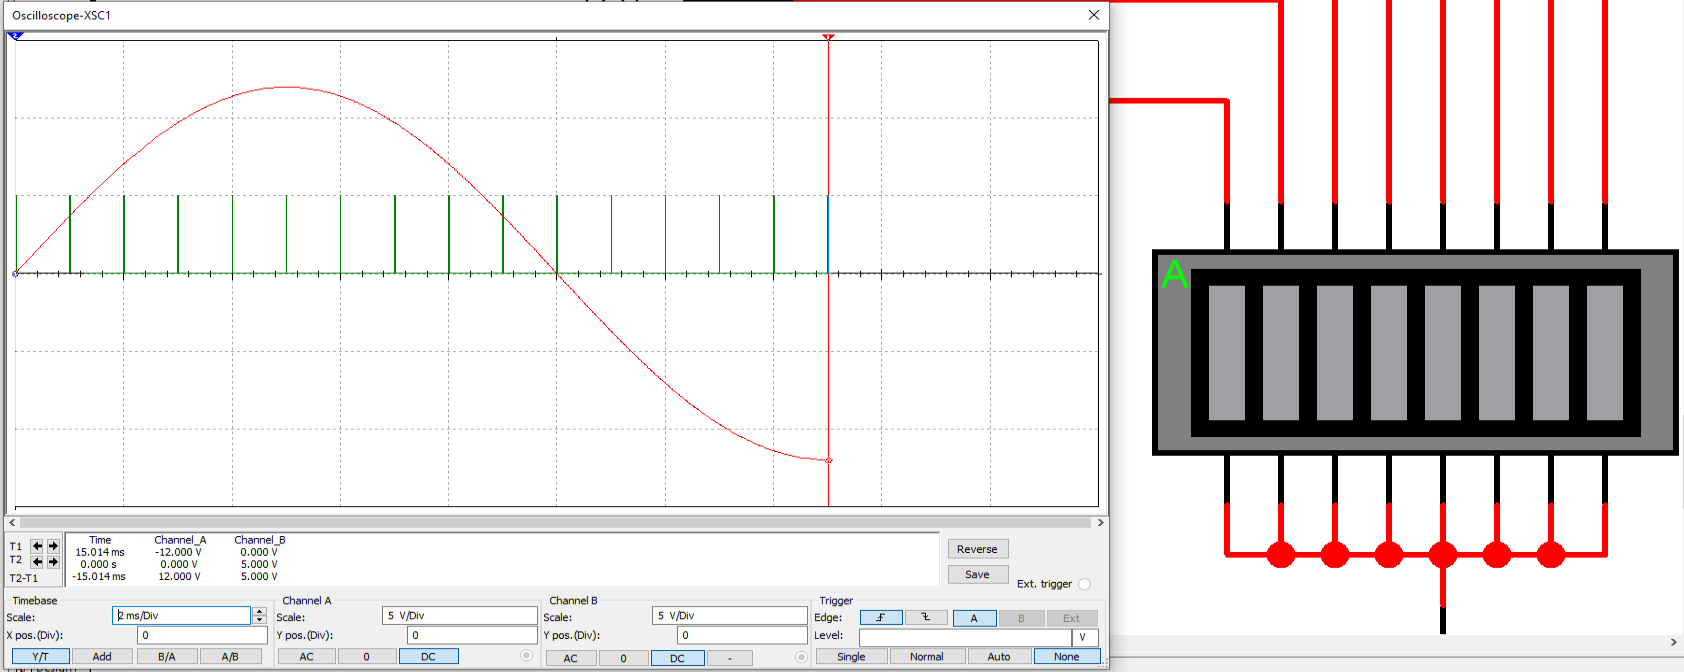
\includegraphics[width=1\textwidth]{Minimo.png}
        \caption{Onda senoidal del Multisim en su pico mas bajo (12V)}
        \label{img:minimo}
    \end{figure}

    El voltaje obtenido de esta medición esta dado por T1 en channel\_A, el cual corresponde al valor de \textbf{-12V} concordando con la configuración establecida en $V_{ref-}$. Los LEDs nos indican que el código binario asignado para los -12V es de \textbf{00000000}  (8 bits apagados), para verificar este código se usara la ecuación \ref{eq:D10}:

    De acuerdo a los datos del diseño:
    \begin{itemize}
        \item Voltaje de entrada: $V_{in} = -12 \text{ V}$
        \item Voltaje de referencia mínimo: $V_{min} = -12 \text{ V}$
        \item Voltaje de resolución: $V_{res} = 0.09375 \text{ V}$
    \end{itemize}

    $$D_{10} = \frac{-12 - (-12)}{0.09375} = \frac{0}{0.09375} = 0$$

    Dado que el resultado decimal es $0$, su representación en un sistema de $8$ bits corresponde a todos los dígitos en estado lógico bajo:

    $$0_{10} = 00000000_2$$

    Este resultado confirma que el ADC está correctamente calibrado con respecto a su voltaje de referencia negativo ($V_{ref-}$), asignando el valor mínimo de la escala digital al límite inferior.

    \subsection{\textit{Caso 3: Punto aleatorio}}

    En este caso, se pausó la simulación cuando la salida mostró una señal analógica arbitraria. El voltaje correspondiente a la mediante esta dado por T2 en channel\_A el cual entrega un valor de \textbf{-3.704V} junto a un código binario de \textbf{01011000}, lo anterior se aprecia en la Figura \ref{img:random}.

    \begin{figure}[H]
        \centering
        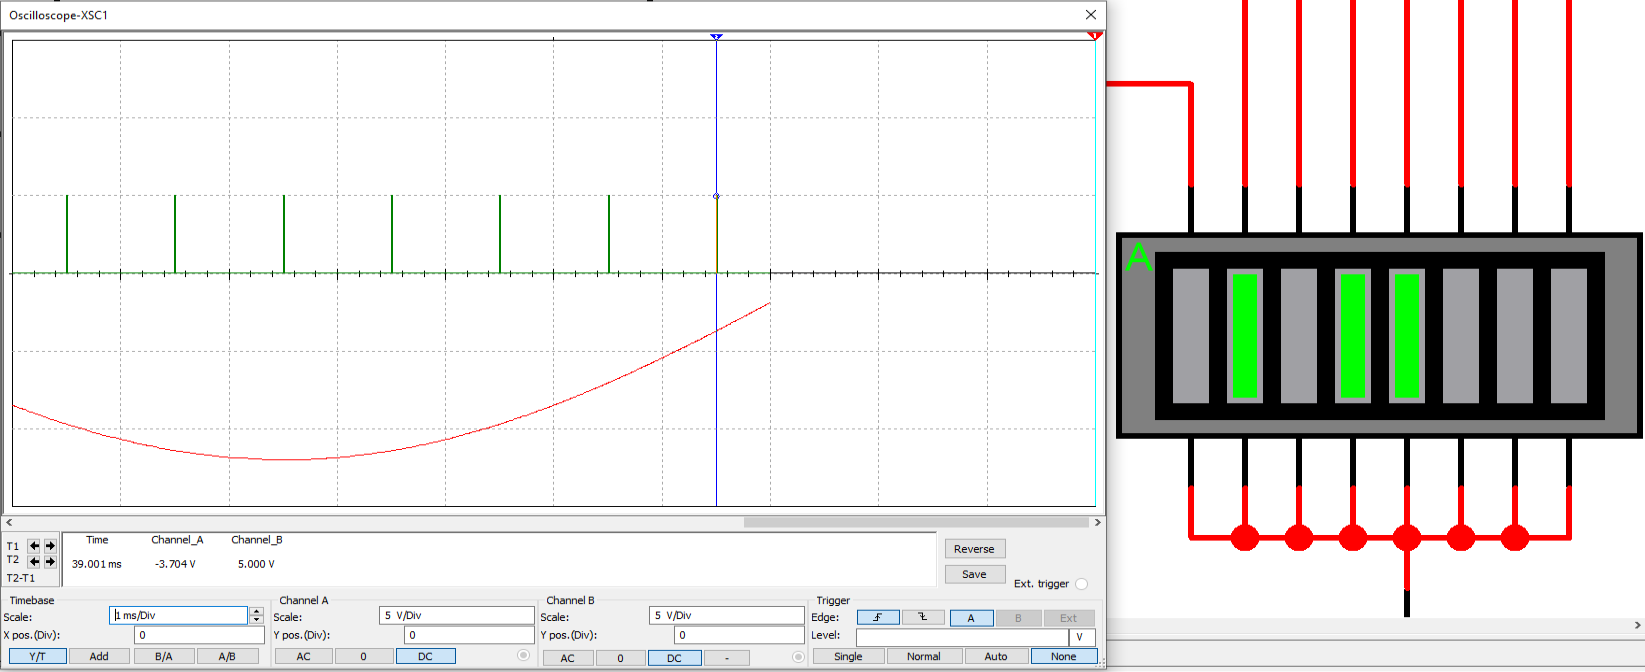
\includegraphics[width=1\textwidth]{Random.png}
        \caption{Onda senoidal del Multisim en un punto arbitrario (12V)}
        \label{img:random}
    \end{figure}

    A diferencia de los casos anteriores, en esta instancia se busca validar el voltaje de entrada ($V_{in}$) a partir del código binario entregado por el ADC en un instante arbitrario de la simulación.

    Los parámetros de diseño se mantienen constantes:
    \begin{itemize}
        \item Voltaje de referencia mínimo: $V_{min} = -12 \text{ V}$
        \item Voltaje de resolución: $V_{res} = 0.09375 \text{ V}$
    \end{itemize}

    $$01011000_2 \Leftrightarrow 88_{10}$$

    Utilizando la ecuación \ref{eq:D10} despejando en función del voltaje de entrada:

    $$V_{in} = (D_{10} \cdot V_{res}) + V_{min} \Rightarrow (88 \cdot 0.09375) + (-12) = -3.75 \text{ V}$$


    El voltaje teórico calculado es de $-3.75 \text{ V}$. Al contrastar este valor con la medición en la Figura \ref{img:random}, la cual entrega un valor de $-3.704 \text{ V}$, se observa una diferencia de apenas $0.046 \text{ V}$.

    Esta discrepancia es inferior al voltaje de resolución calculado (0.09375V) y se sitúa dentro del margen del error de cuantización ($\pm 0.046875 \text{ V}$), lo que confirma que el ADC está asignando correctamente los niveles discretos.


    \newpage
    
    \section{Conclusión}

    El laboratorio permitió culminar de manera exitosa el estudio y la implementación simulada en un Convertidor analógico-Digital(ADC), un componente fundamental para la arquitectura de sistemas informáticos modernos y el procesamiento de señales empíricas. a lo largo del desarrollo teórico y práctico, se evidencio empíricamente como las magnitudes físicas continuas,que varían de manera infinita en el tiempo, pueden ser traducidas a un lenguaje discreto.posibilitando su procesamiento y almacenamiento en sistemas digitales computacionales.


    Comenzando por la implementación del teorema de Nyquist que demostró ser un pilar clave para la viabilidad del proceso de discretización. Al trabajar bajo una señal analógica de entrada senoidal con una frecuencia de de 50hz, se establece un muestro a una frecuencia de un 1khz esto permitió un total de 20 muestras por ciclo. Esta relación de diseño superó holgadamente el requisito mínimo teórico de muestrear al menos al doble de la frecuencia máxima de la señal, asegurando de esta manera una representación precisa de la onda y mitigando así el riesgo de posibles pérdidas de información o distorsión estructural durante el proceso.

    Por otra parte, el proceso de de cuantificación facilitó comprender las limitaciones de precisión que son inherentes a los componentes de hadware. Al implementar un ADC de 8 bits para un rango de operación comprendiendo entre -12v y 12v, el sistema entrego una capacidad de 256 niveles discretos. Esto se tradujo directamente en un voltaje de resolución exacto de 0.09375V por cada incremento binario. Este valor se determina como el “escalón” de digitalización e ilustra físicamente la fidelidad de la conversión. El diseño de sistemas que convierten señales analógicas a digitales enfrenta un error de cuantización inevitable, equivalente a la mitad del voltaje de resolución. Aunque en este caso se logra una precisión adecuada, la teoría indica que aumentar los bits del convertidor reduce este error, mejorando la fidelidad de la reconstrucción de la señal original. Es crucial entender este margen de error al diseñar sistemas informáticos, ya que la calidad de los datos digitalizados influye en la fiabilidad del software, evitando errores causados por lecturas imprecisas.

    La simulación realizada bajo condiciones ideales validó completamente el desarrollo matemático previo. Se logró transformar un voltaje analógico de 2.5 V en un tren de pulsos visible a través de LEDs, con un valor cuantificado de 154 que corresponde a la salida binaria 10011010. La coincidencia entre los resultados teóricos y empíricos obtenidos en la simulación en Multisim confirma el óptimo funcionamiento del diseño sistémico.

    En síntesis, este laboratorio validó los principios de digitalización y demostró que integrar la teoría y simulación previa ante cualquier implementación física es de suma importancia. Dominar los conversores ADC, sus resoluciones y frecuencias de muestreo, resulta indispensable para el desarrollo de sistemas informáticos capaces de procesar e interpretar las variaciones continuas que conlleva el mundo físico. 

    \newpage
    \printbibliography
    \nocite{*}

    \section{Anexo}

    Tabla de cuantización del ADC de 8 bits (256 niveles):
    \\
    \footnotesize \url{https://docs.google.com/spreadsheets/d/1Zy71eyLFHjzah7Zh_w69UBaSy9Q9xg6tVxTYqCIr43Q/edit?usp=sharing}

\end{document}